\chapter{The Technology File: Where Physics Becomes Rules}

\begin{tldr}
\begin{itemize}
  \item \textbf{Last chapter:} the SDC turned a netlist into a timed promise every tool measures against. \textbf{This chapter:} the tech file is the foundry rulebook every routed shape must obey before that promise can be cashed in silicon.
  \item The \textbf{technology file} is the foundry contract that turns silicon physics into machine-readable design rules your PD tool obeys layer by layer.
  \item It carries \textbf{layer definitions, min width/spacing, min area, via geometries, sheet resistance, thickness, permittivity, and colors} for multi-patterning.
  \item Without it, the router has \textbf{no legal moves}: every wire it draws would be a DRC violation waiting to happen.
  \item Two cousins exist in real flows: the older Cadence \texttt{.tf} format and the modern \textbf{tech-LEF} abstraction, often paired with an \texttt{ITF} for parasitic extraction.
\end{itemize}
\end{tldr}

\begin{hook}
Imagine handing a contractor a blueprint with no building code, no minimum stud spacing, no fire rating, no permitted materials. He builds whatever he wants and the inspector burns it down. That is exactly what a place-and-route tool would do without a tech file, except the inspector is the foundry mask shop and \enquote{burning it down} means a \$3M tapeout that yields zero working die. So how does a four-kilobyte ASCII file save a multi-million-dollar wafer run?
\end{hook}

\section{The Stack You Are Actually Routing On}

A modern CMOS chip is a sandwich of conducting metal layers separated by dielectric, stitched together by tiny vertical plugs called vias. The tech file describes \textbf{every one of those layers}, bottom to top, with the numbers a router needs to keep wires legal and signals fast. Layers near the substrate are \textbf{thin and tight} (good for short local nets, bad for current); layers up top are \textbf{thick and wide} (good for power and clock, bad for density).

\begin{figure}[h]
\centering
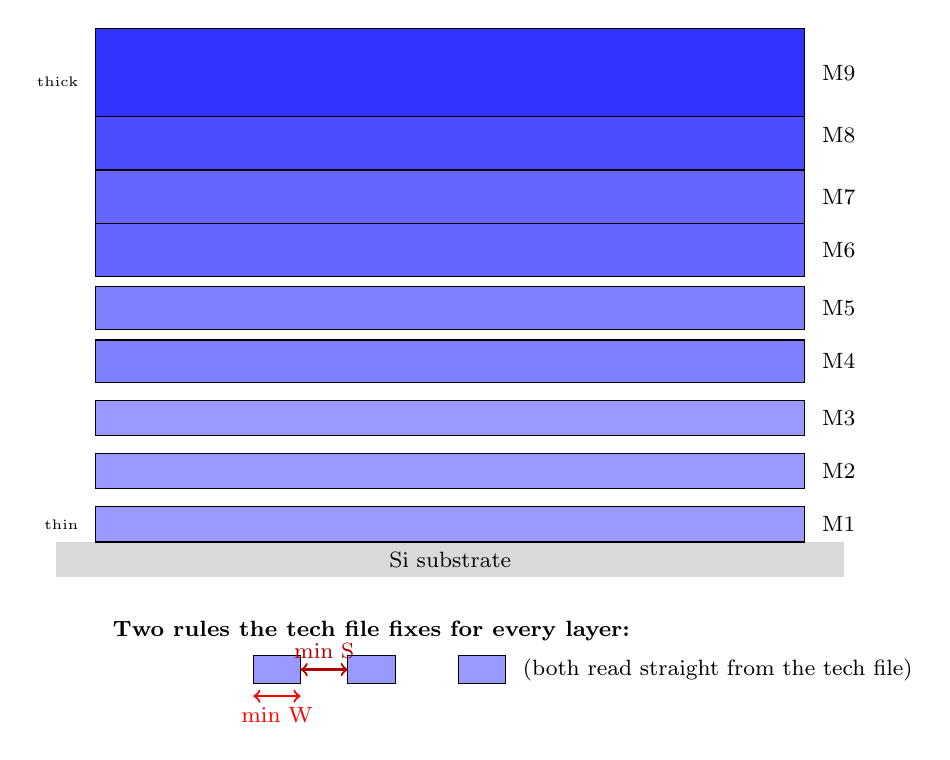
\begin{tikzpicture}[x=1cm,y=0.45cm]
  % substrate
  \fill[gray!30] (0,0) rectangle (10,1); \node at (5,0.5) {\footnotesize Si substrate};
  % metal stack alternating dielectric (light) and metal (dark)
  \foreach \i/\name/\h/\col in {
    1/M1/1.0/blue!40,
    2/M2/1.0/blue!40,
    3/M3/1.0/blue!40,
    4/M4/1.2/blue!50,
    5/M5/1.2/blue!50,
    6/M6/1.5/blue!60,
    7/M7/1.5/blue!60,
    8/M8/2.0/blue!70,
    9/M9/2.5/blue!80
  }{
    \pgfmathsetmacro{\ybot}{1 + (\i-1)*1.5}
    \fill[\col] (0.5,\ybot) rectangle (9.5,\ybot+\h);
    \draw (0.5,\ybot) rectangle (9.5,\ybot+\h);
    \node[right] at (9.6,\ybot+\h/2) {\footnotesize \name};
  }
  % min width / min spacing callout: drawn as a separate inset below the stack
  \begin{scope}[shift={(2.5,-3.0)}]
    \node[font=\footnotesize\bfseries] at (1.5,1.5) {Two rules the tech file fixes for every layer:};
    \fill[blue!40] (0.0,0) rectangle (0.6,0.8); \draw (0.0,0) rectangle (0.6,0.8);
    \fill[blue!40] (1.2,0) rectangle (1.8,0.8); \draw (1.2,0) rectangle (1.8,0.8);
    \draw[<->,thick,red] (0.0,-0.35) -- (0.6,-0.35);
    \node[below,font=\footnotesize\color{red}] at (0.3,-0.38) {min W};
    \draw[<->,thick,red!70!black] (0.6,0.4) -- (1.2,0.4);
    \node[above,font=\footnotesize\color{red!70!black}] at (0.9,0.45) {min S};
    \fill[blue!40] (2.6,0) rectangle (3.2,0.8); \draw (2.6,0) rectangle (3.2,0.8);
    \node[right,font=\footnotesize] at (3.3,0.4) {(both read straight from the tech file)};
  \end{scope}
  \node[left] at (0.4,1.5) {\tiny thin};
  \node[left] at (0.4,14) {\tiny thick};
\end{tikzpicture}
\caption{Metal stack M1 through M9. Lower layers are thin and dense; upper layers grow thicker for current handling. The red arrows on M2 show the two rules the tech file enforces everywhere: minimum width and minimum spacing.}
\end{figure}

\begin{keyidea}
The technology file is the \textbf{foundry-supplied rulebook} that names every physical layer, fixes its geometric and electrical parameters, and tells the PD tool exactly what shapes it is allowed to draw.
\end{keyidea}

\section{What Lives Inside the File}

Open a real tech file and you will see a layered structure: chip-level parameters first (chip X/Y, frequency, FFT area for RF flows), then a substrate and dielectric block, then a long tail of \textbf{metal and via blocks}. Each metal entry carries a layer number, a name, a color, sheet resistance, thickness, and the design rules that come with it. The dielectric entries carry \textbf{permittivity} (relative, unitless) and \textbf{thickness} in microns, because that is what an extractor needs to back out capacitance.

\begin{figure}[h]
\centering
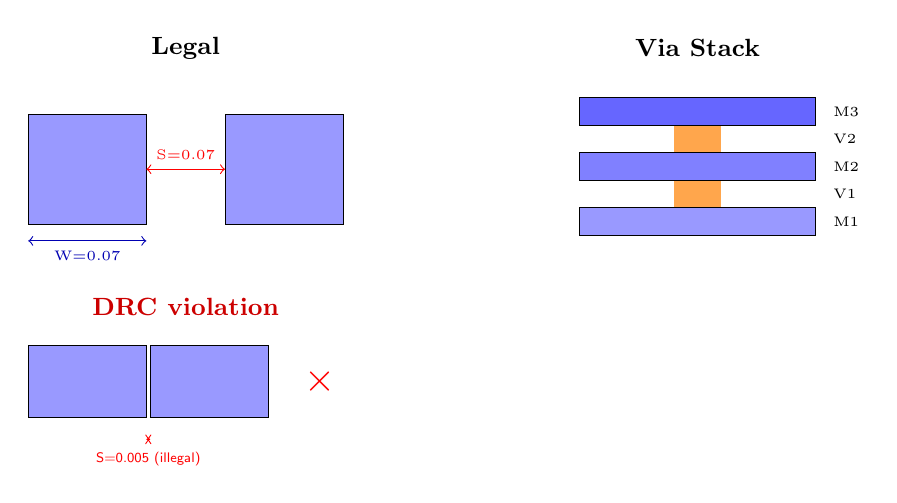
\begin{tikzpicture}[x=1cm,y=0.7cm]
  % LEFT: good spacing
  \node[font=\small\bfseries] at (2.5,5.2) {Legal};
  \fill[blue!40] (0.5,2) rectangle (2.0,4);
  \fill[blue!40] (3.0,2) rectangle (4.5,4);
  \draw (0.5,2) rectangle (2.0,4);
  \draw (3.0,2) rectangle (4.5,4);
  \draw[<->,red] (2.0,3) -- (3.0,3) node[midway,above,font=\tiny\color{red}]{S=0.07};
  \draw[<->,blue!70!black] (0.5,1.7) -- (2.0,1.7) node[midway,below,font=\tiny]{W=0.07};
  % via stack overlay on right column
  \node[font=\small\bfseries] at (9,5.2) {Via Stack};
  \fill[blue!40] (7.5,1.8) rectangle (10.5,2.3); \node[right,font=\tiny] at (10.6,2.05){M1};
  \fill[orange!70] (8.7,2.3) rectangle (9.3,2.8); \node[right,font=\tiny] at (10.6,2.55){V1};
  \fill[blue!50] (7.5,2.8) rectangle (10.5,3.3); \node[right,font=\tiny] at (10.6,3.05){M2};
  \fill[orange!70] (8.7,3.3) rectangle (9.3,3.8); \node[right,font=\tiny] at (10.6,3.55){V2};
  \fill[blue!60] (7.5,3.8) rectangle (10.5,4.3); \node[right,font=\tiny] at (10.6,4.05){M3};
  \draw (7.5,1.8) rectangle (10.5,2.3);
  \draw (7.5,2.8) rectangle (10.5,3.3);
  \draw (7.5,3.8) rectangle (10.5,4.3);
  % DRC violation row
  \node[font=\small\bfseries\color{red!80!black}] at (2.5,0.5) {DRC violation};
  \fill[blue!40] (0.5,-1.5) rectangle (2.0,-0.2);
  \fill[blue!40] (2.05,-1.5) rectangle (3.55,-0.2);
  \draw (0.5,-1.5) rectangle (2.0,-0.2);
  \draw (2.05,-1.5) rectangle (3.55,-0.2);
  \draw[<->,red] (2.0,-1.9) -- (2.05,-1.9);
  \node[font=\tiny\color{red},below] at (2.025,-1.95) {\textsf{S=0.005 (illegal)}};
  \node[font=\Large\bfseries\color{red}] at (4.2,-0.85) {$\boldsymbol{\times}$};
\end{tikzpicture}
\caption{Left: two M2 wires with the legal minimum spacing the tech file declares. Right: a via stack M1$\to$V1$\to$M2$\to$V2$\to$M3 with the vias defined as small square cuts inside larger metal landing pads. Bottom: the same two wires drawn too close, which the DRC engine flags instantly because the spacing rule was read straight from the tech file.}
\end{figure}

\begin{lstlisting}[style=eda,caption={Skeleton of a tech file fragment (illustrative)}]
chip_x = 1200
chip_y = 1200
tech_file = "rf28_v1.tf"
frequency = 2.4e9
layer substrate { rho = 10  ; thickness = 280 }
layer ild1      { eps_r = 4.2 ; thickness = 0.4 }
layer metal0    { num=1 ; rs=0.12 ; t=0.13 ; color=red    ; minW=0.07 ; minS=0.07 }
layer metal1    { num=2 ; rs=0.10 ; t=0.15 ; color=green  ; minW=0.07 ; minS=0.07 }
via   v1        { from=metal0 ; to=metal1 ; cut=0.07x0.07 ; enc=0.005 }
\end{lstlisting}

\subsection*{Memory hooks}

\begin{pdnote}
\textbf{Hook 1.} The \textbf{foundry stapler} \textit{slams} the rulebook onto your desk; lose it and your router \textit{flies blind into a million-dollar wall}.

\textbf{Hook 2.} \textbf{Dielectric layers} \textit{whisper} their permittivity to the \textbf{extractor}; misread them and your \textit{timing report lies to your face}.
\end{pdnote}

\subsection*{Gut checks}

\begin{gut}
You delete the via definition for V3 from the tech file and rerun routing. What breaks first? \gutans{The router cannot legally connect M3 to M4, so any net needing that transition fails (open net or DRC) and the tool errors out before completing.}
\end{gut}

\begin{gut}
Why is M9 drawn three times thicker than M1 in the stack figure? \gutans{Upper metals carry power and global clock; thicker metal lowers sheet resistance and IR drop. Lower metals stay thin to keep pitch tight for dense local routing.}
\end{gut}

\begin{pausebox}
Stop. Before reading on, predict: if a tech file lists \textbf{only} M1 through M5 but your floorplan needs a top-level clock mesh, what happens when you try to route the mesh on M6? Say it out loud.
\end{pausebox}

\section{Worked Example: Counting Tracks Across a Channel}

\textbf{Setup.} M2 has \textbf{min width $W = 0.07\,\mu m$} and \textbf{min spacing $S = 0.07\,\mu m$}. A routing channel is \textbf{5.0 microns wide}. How many M2 tracks fit?

\move{1} Substitute the numbers into the pitch definition:
\[
\text{pitch} = W + S = 0.07 + 0.07 = 0.14\,\mu m.
\]

\move{2} Divide the available channel width by the pitch:
\[
N = \left\lfloor \frac{5.0}{0.14} \right\rfloor = \lfloor 35.71 \rfloor = 35 \text{ tracks}.
\]

\move{3} Sanity check by rebuilding the total occupied width:
\[
35 \times 0.14 = 4.90\,\mu m \le 5.0\,\mu m. \checkmark
\]

\move{4} The leftover $0.10\,\mu m$ is not enough for a 36th track (would need another $0.14\,\mu m$), so 35 is tight and correct.

\begin{keyidea}
\textbf{Routing capacity per layer} is set entirely by the tech file. Change \textbf{minW} or \textbf{minS} by ten nanometers and your channel either fits the design or fails routing congestion.
\end{keyidea}

\section{Watch Out}

\begin{pitfall}
\textbf{Tech file vs tech-LEF.} They are siblings, not twins. The Cadence \texttt{.tf} is the older, richer foundry-format file (often paired with an \texttt{ITF} for extraction). \textbf{tech-LEF} is the LEF/DEF-style abstraction modern Synopsys and tool-agnostic flows consume. Some tools accept either depending on the flow; do not assume one is a drop-in replacement for the other. Always match the tech format to what your PnR tool expects in its reference flow doc.
\end{pitfall}

\begin{pitfall}
\textbf{Colors are not just metal names.} At advanced nodes (sub-20nm), the \texttt{color} field is not cosmetic. It encodes \textbf{mask assignment for multi-patterning}. Two same-color shapes that are too close are a \textbf{coloring violation}, distinct from a normal spacing DRC. Treat color as a hard physical attribute, not a label.
\end{pitfall}

\begin{sidebar}{Why advanced nodes make this file explode}
At 7nm and below, a single metal layer is printed across \textbf{multiple masks} (LELE, SADP, SAQP). The tech file now has to declare \textbf{decomposition rules}, \textbf{coloring constraints}, \textbf{cut-mask geometries}, and per-color minimum spacings. A 28nm tech file might be a few thousand lines; a 5nm tech file plus its rule decks pushes into the hundreds of thousands. The discipline is the same, the size is not.
\end{sidebar}

\begin{pdnote}
\textbf{Why PD cares (three lenses):}
\begin{itemize}
  \item \textbf{Arm PD intern:} You will never write a tech file, but on day one you will load one and \texttt{grep} it for layer counts, min pitches, and via definitions to sanity check your floorplan.
  \item \textbf{Generic foundry PD engineer:} You consume the PDK as ground truth. When a router complains \enquote{no legal via found,} the answer is in the tech file's via section nine times out of ten.
  \item \textbf{VLSI interview:} \enquote{What is in a tech file and why do you need it?} is a layup question. Name layer defs, design rules, vias, RC parameters, and units. Bonus points for distinguishing \texttt{.tf} from tech-LEF.
\end{itemize}
\end{pdnote}

\begin{checkpoint}
\textbf{You should now be able to:}
\begin{itemize}
  \item Name at least five categories of information stored in a tech file.
  \item Compute routing pitch and tracks per channel from min width and min spacing.
  \item Explain the difference between \texttt{.tf} and tech-LEF in one sentence.
  \item Say why coloring fields stop being decorative at advanced nodes.
\end{itemize}

\mnemonic{\textbf{LIVR-C}: \textbf{L}ayers, \textbf{I}LD/permittivity, \textbf{V}ias, \textbf{R}ules (W/S/area), \textbf{C}olors. Five buckets, one file, every PD flow.}
\end{checkpoint}
